\documentclass[a4paper]{article}
\usepackage[warn]{mathtext}
\usepackage[utf8]{inputenc}
\usepackage[T2A]{fontenc}
\usepackage[english,russian]{babel}
\usepackage{booktabs}
\usepackage{multicol}
\usepackage{fancyhdr}
\usepackage{graphicx}
\usepackage{microtype}
\usepackage{wrapfig}
\usepackage{amsmath}
\usepackage{floatflt}
\usepackage{geometry} \geometry{verbose,a4paper,tmargin=2cm,bmargin=2cm,lmargin=1.5cm,rmargin=1.5cm}
\usepackage{float}
\usepackage{amssymb}
\usepackage{caption}
\usepackage{epsfig}
\usepackage{newunicodechar}

\begin{document}

\graphicspath{ {pictures/} }
\begin{center}
    {\scshape\Large Лабораторная работа по твердотельной электронике} \par

    \

    {\huge\bfseries № 3. Определение ширины запрещенной зоны полупроводников} \par 

    \

    {\large Яромир Водзяновский Б04-855а}
    {\large Данила Буданый}
\end{center}

\

\
\textbf{Цель работы:} Определение ширины запрещённой зоны материала фоторезистора (CdSe) по спектральной зависимости собственной фотопроводимости.

\section{Эксперимент}

Получили зависимость сигнала относительного фотоответа от энергии


\begin{figure}[H]
    \centering
    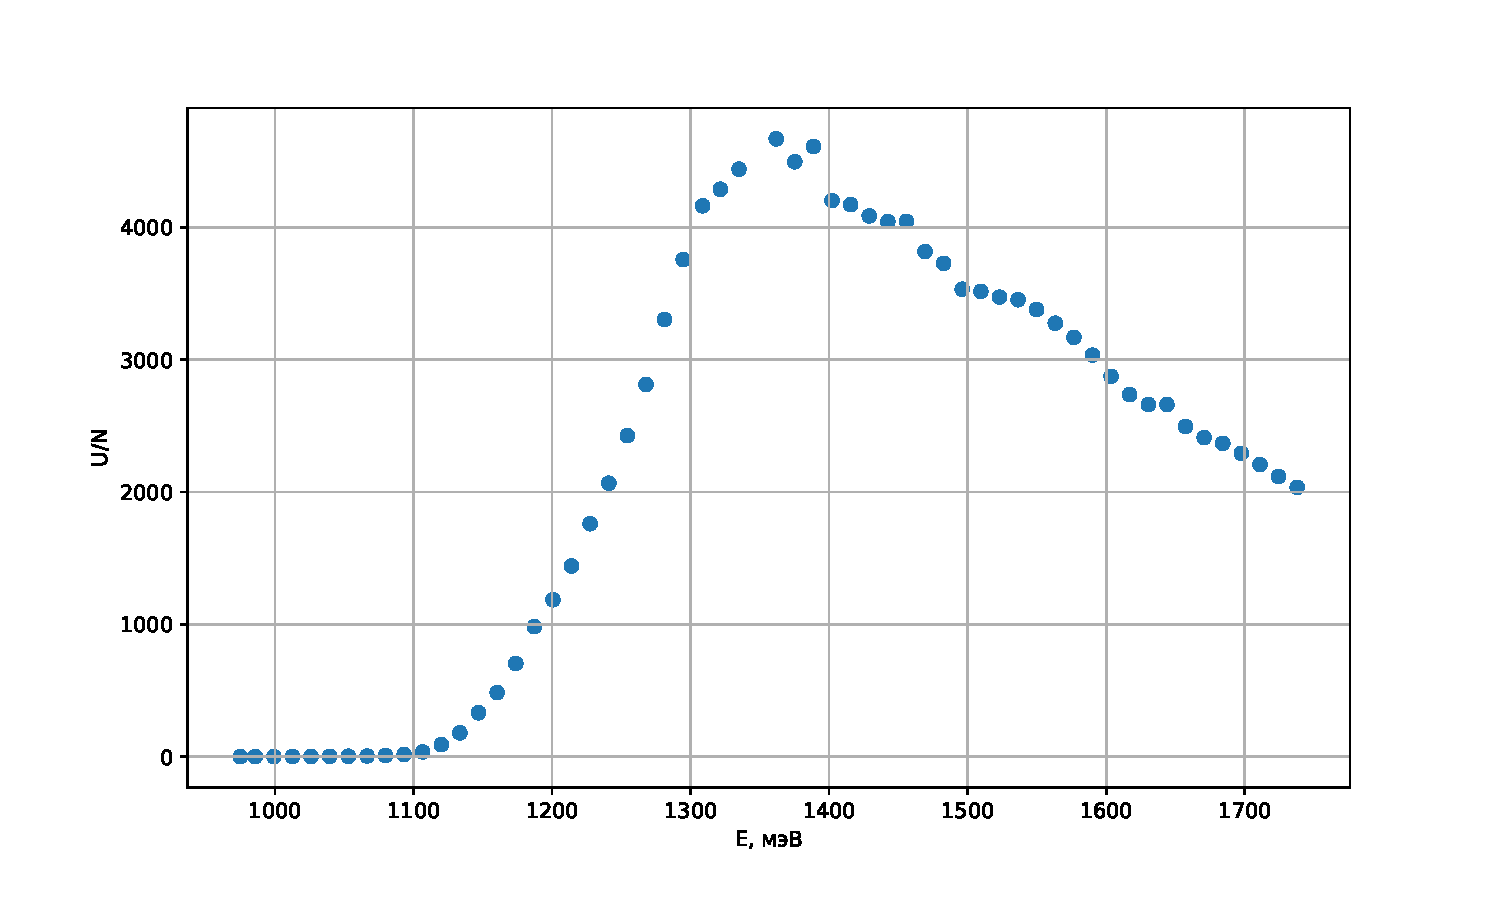
\includegraphics[scale = 0.5]{gr2.pdf}
    \caption{}
    \label{gr2}
\end{figure} 

\begin{figure}[H]
    \centering
    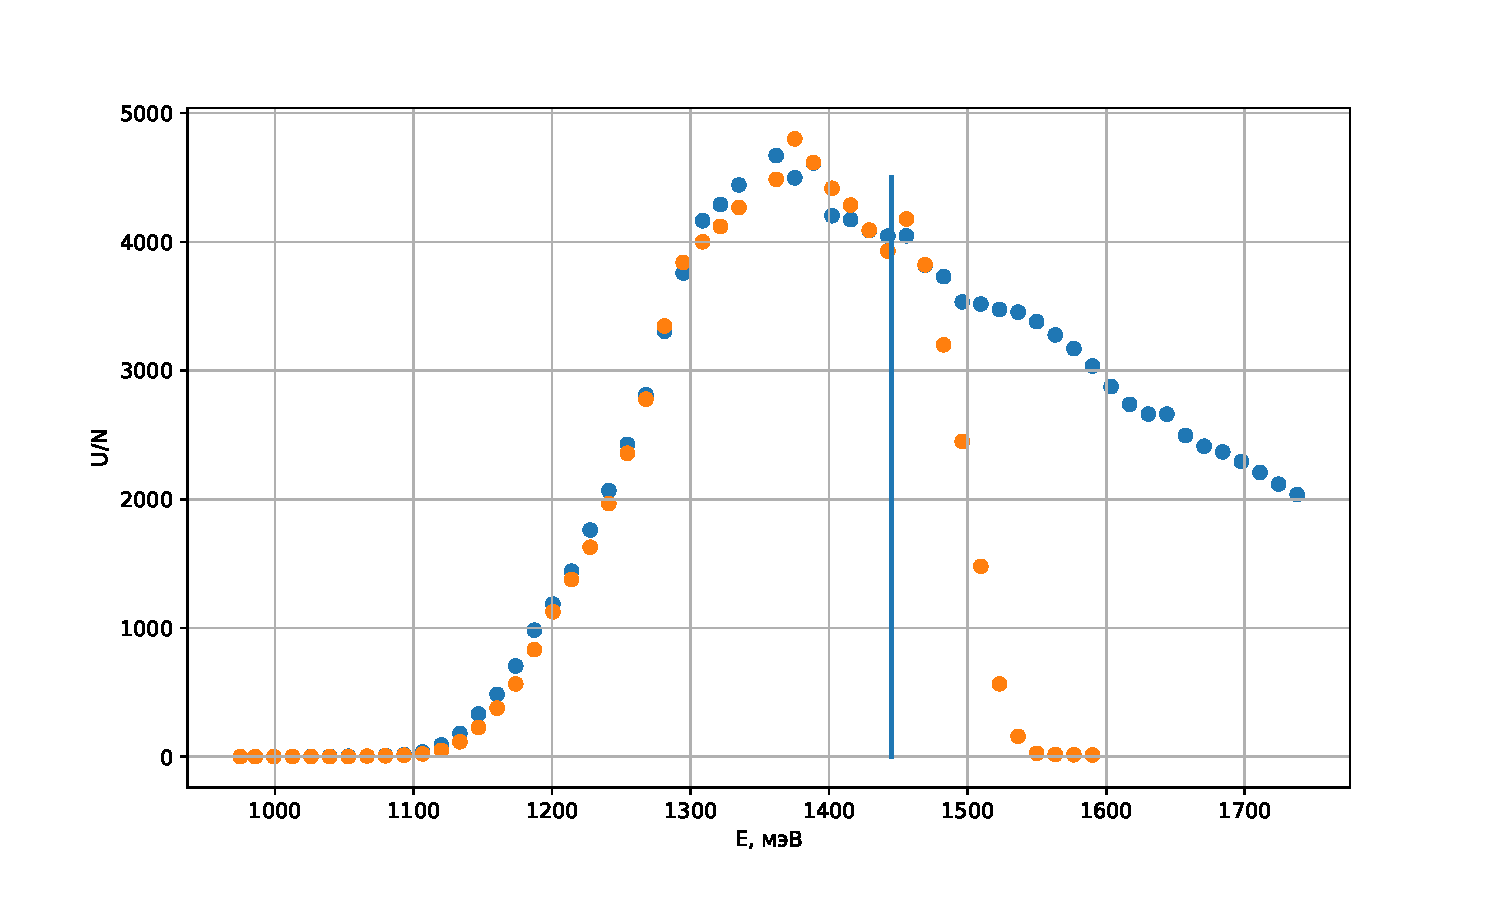
\includegraphics[scale = 0.5]{gr3.pdf}
    \caption{}
    \label{gr3}
\end{figure} 



Определим энергию фонона и ширину запрещенной зоны с добавлением аппроксимации и дальнейшей математической экстраполяции в области малой оптической толщины ($Kd \ll 1 $) рис \ref{gr1}

\begin{figure}[H]
    \centering
    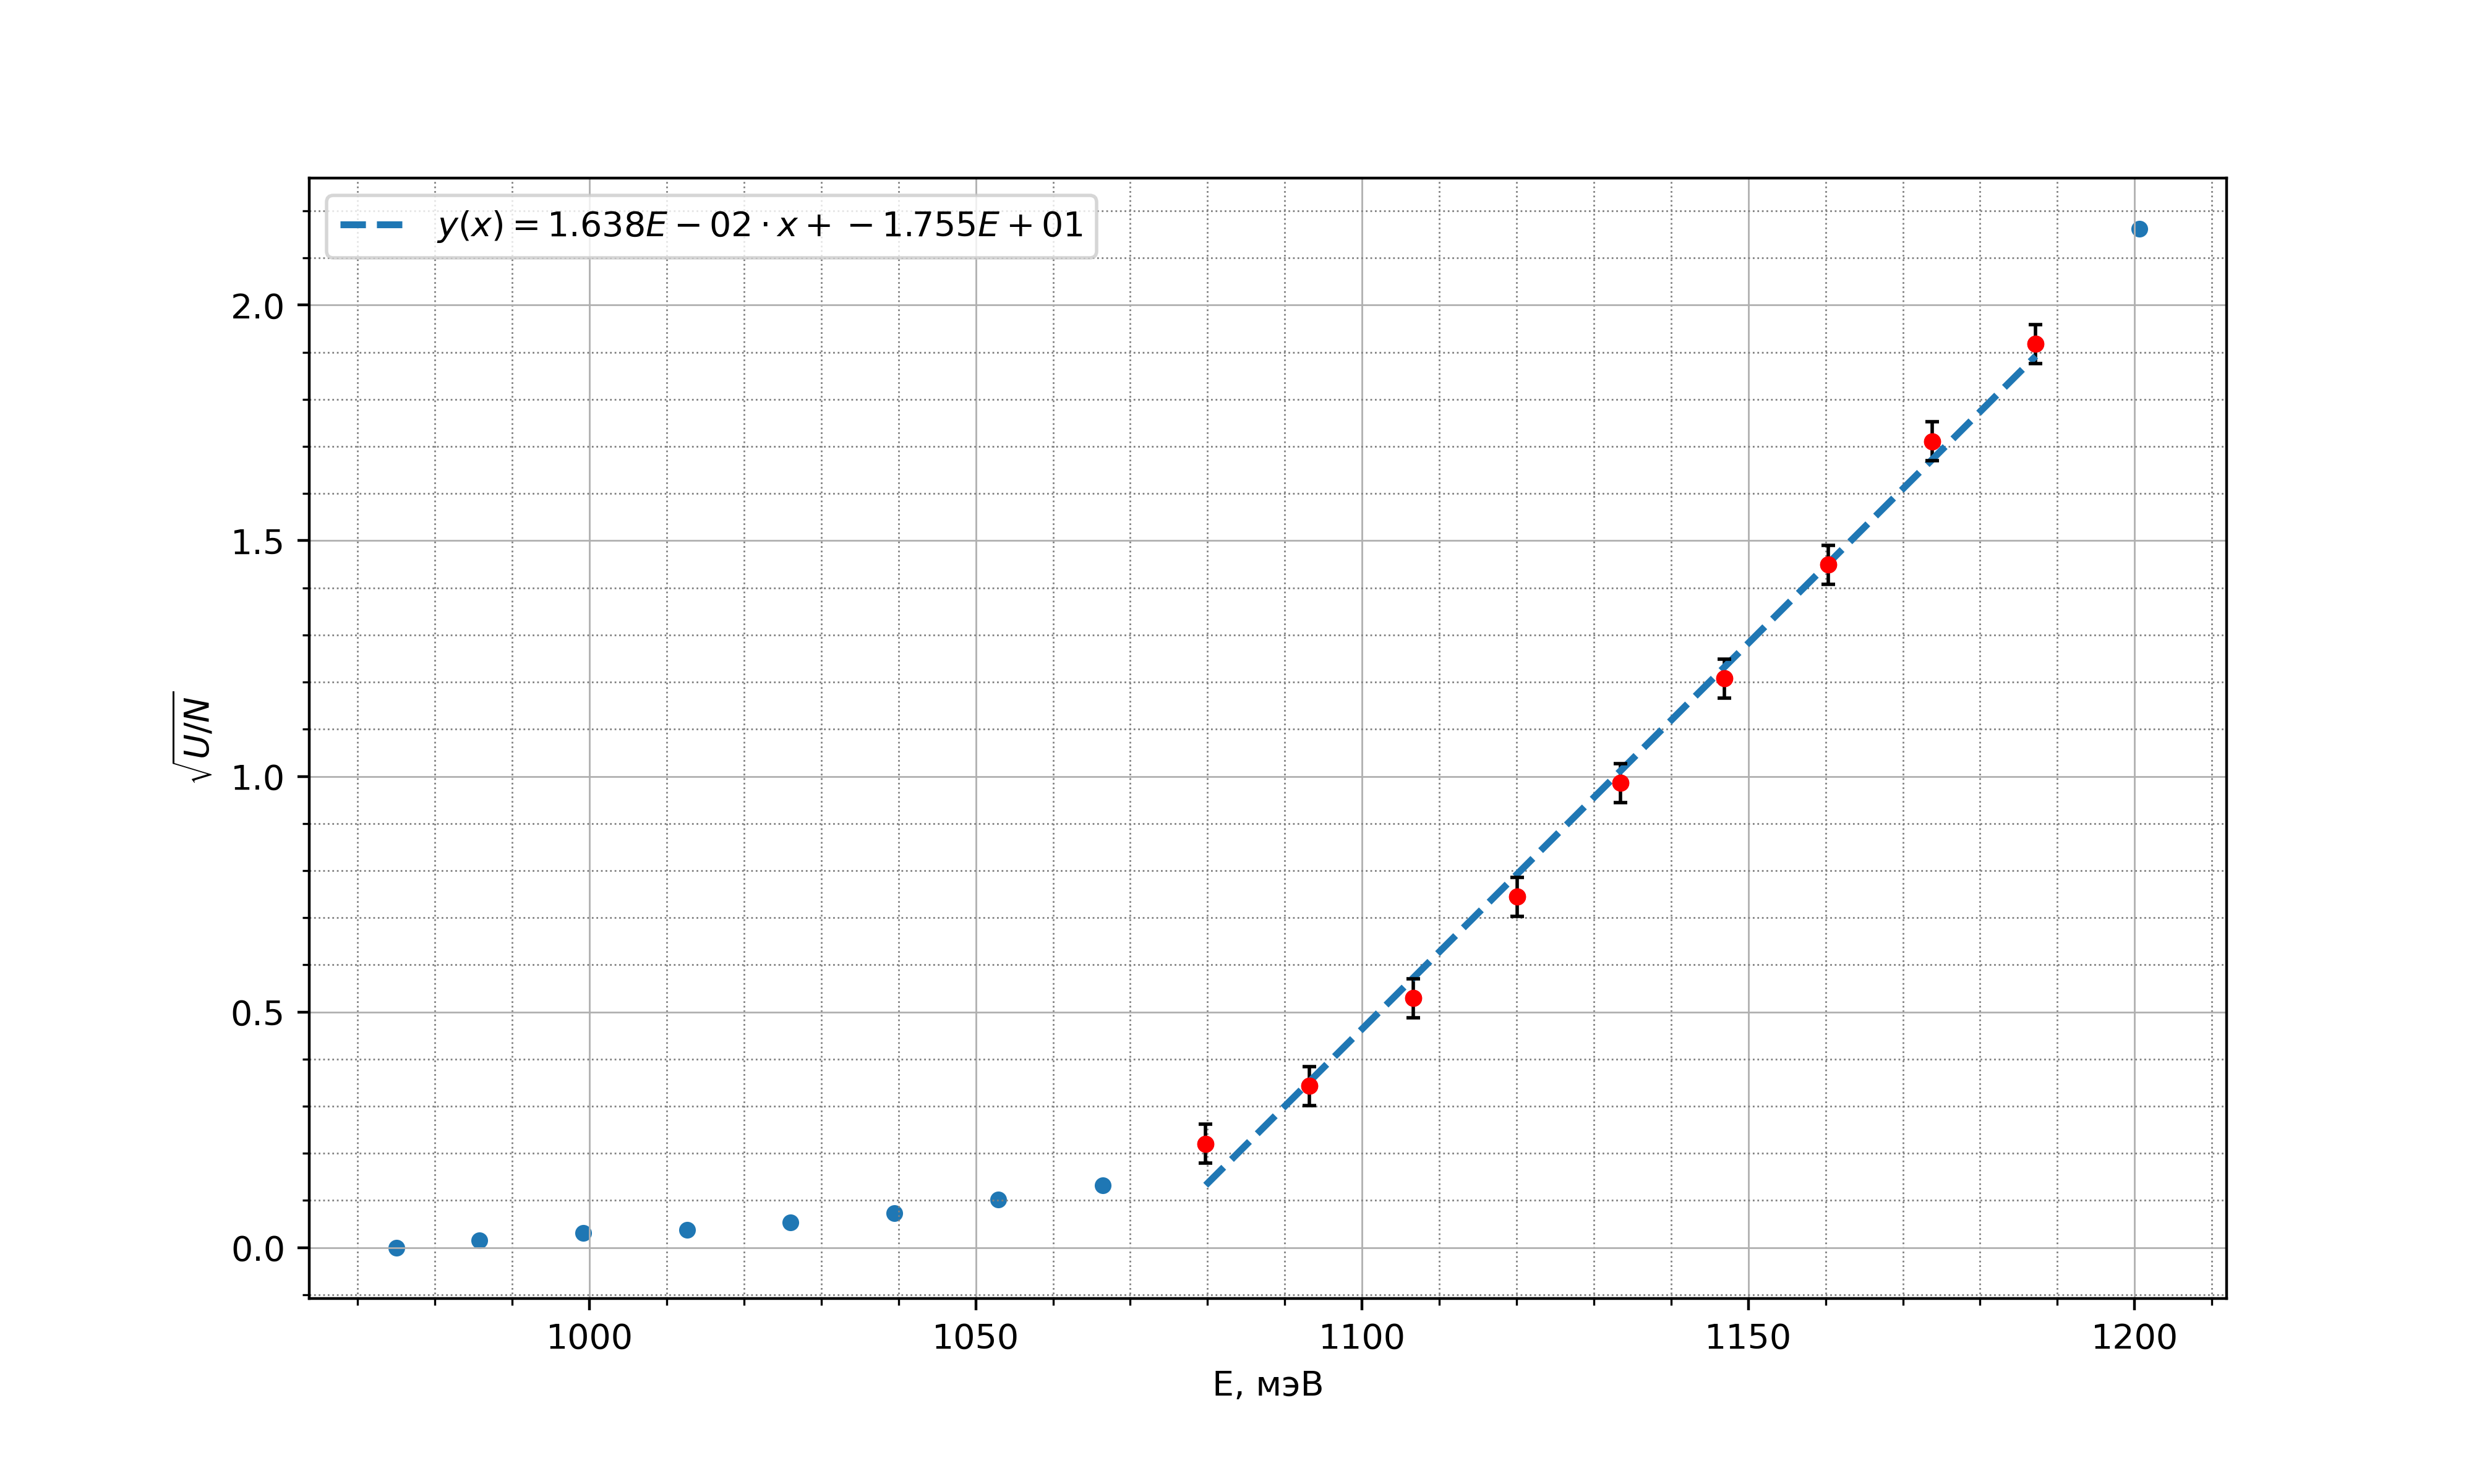
\includegraphics[scale = 0.6]{gr1.png}
    \caption{}
    \label{gr1}
\end{figure} 
Энергия фонона равна $50$ мэВ. Ширина запрщенной зоны 1071 мэВ

\section{Вопросы}

\begin{enumerate}
    \item Что такое скорость оптической генерации? Её размерность? \par 
    Cкоростью оптической генерации называют количество пар электронов и дырок, появляющихся в единице объёма за единицу времени. Таким образом размерность скорости оптической генерации – $[g] = c^{-1} \cdot м^{-3}$.

    \item Разъяснить понятие «оптически тонкий образец» \par 
    В случае, когда скорость оптической генерации слабо изменяется в направлении освещения, говорят, что образец является оптически тонким. Это утверждение аналогично тому, что поглощение света в образце очень слабое. Математическое утверждение выглядит следующим образом:
    $g \sim e^{-Kx}$ , где К – коэффициент поглощения. Отсюда следует, что образец называется оптически тонким при выполнении условия $Kd \ll 1$ 

    \item  Получить выражение для скорости оптической генерации в случае, когда образец можно считать оптически тонким. \par 
    $$g(x) = \beta \frac{KN_0 (1-R)}{1 - R^2 e^{-2Kd}} (e^{-Kx} + Re^{-K(2d-x)})$$
    При малой оптической толщине $kd<<1$. Для $\beta \approxeq 1$
    $$g(x) \approxeq \frac{KN_0(1-R)}{1-R^2(1-2Kd)} ((1-Kx) + R(1-2Kd + Kx))$$
    $$g(x) \approxeq \frac{KN_0 (1-R)}{(1-R)^2} (1+R) = KN_0$$

    \item Как зависит фотопроводимость от коэффициента поглощения при энергиях света, когда образец можно считать оптически тонким? Оптически толстым? \par
    \begin{enumerate}
        \item Опт. тонкий \par 
        Из $\Delta n = \Delta p$ - условие электронейтральности вытекает $\tau_n = \tau_p = \tau$:
        $$\Delta \Sigma = \frac{e(\mu_n + \mu_p) \omega}{l} K(h\nu) N_0 \tau$$
        $$\Delta \Sigma \sim KN_0\tau$$

        \item Опт. толстый \par 
        При $g \approxeq K(1-R)N_0 e^{-Kx}$
        $$\Delta \Sigma \sim \frac{N_0}{\tau}$$
    \end{enumerate}

    \item Рассчитать коэффициент пропорциональности между энергией кванта света в эВ и соответствующей длиной волны в мкм.\par 
    $E = h \nu = h \frac{c}{\lambda} \longrightarrow \lambda E = hc = const \Longrightarrow$ 1 эВ $\Leftrightarrow$ 1.240 мкм.

    \item Ширина зоны прямозонного полупроводника 0,8 эВ. При какой длине волны (в мкм) на фоторезисторе из такого материала можно наблюдать собственную  фотопроводимость? \par 
    $\lambda E = hc = 1.240$ (мкм эВ) $\longrightarrow$ $\lambda = 1.5$ мкм

    \item Темновое сопротивление фоторезистора составляет 40 кОм. Как и какое нагрузочное сопротивление надо припаять в схему для регистрации фотопроводимости, чтобы получить максимальный сигнал? \par 
    $$\Delta u = \varepsilon \frac{R_n R_o}{(R_n + R_o)} \frac{\Delta \Sigma}{\Sigma_o}$$
    $$\Delta u = \varepsilon \frac{R_o^2}{(R_n + R_o)^2} \Delta \Sigma R_n \rightarrow \frac{\partial \Delta u}{\partial R_n} = 0$$
    $$R_n = R_o = 40\; k\Omega$$

    \item На какое расстояние успеют продиффудировать избыточные электроны в Si, если время жизни носителей составляет 10-4 с? \par 
    

    \item На рис.\ref{9} показаны спектральные зависимости фотопроводимости CdS  и CdSe. Пунктирные и сплошные линии соответствуют разным температурам. Какие линии  каким температурам соответствуют? \par 
    \begin{figure}[H]
        \centering
        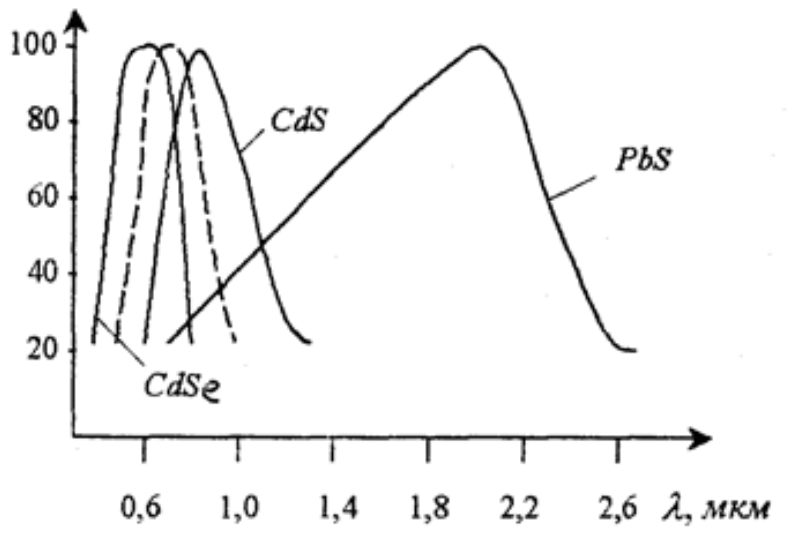
\includegraphics[scale = 0.6]{9.png}
        \caption{}
        \label{9}
    \end{figure} 

    \item Нарисуйте качественно зависимость сигнала фотопроводимости кремниевого фоторезистора от энергии кванта. Энергия фонона  50 мэВ. \par 

    \item Как зависит фотопроводимость U/N при Kd1 от $h \nu$ в прямозонных полупроводниках? \par 

    \item  На рис.\ref{12} приведены результаты измерения сигнала  U фотопроводимости (ФП) образца CdSe  в зависимости от энергии $h \nu$ падающего на образец света. Этот ПП – прямозонный. \par 
    \begin{figure}[H]
        \centering
        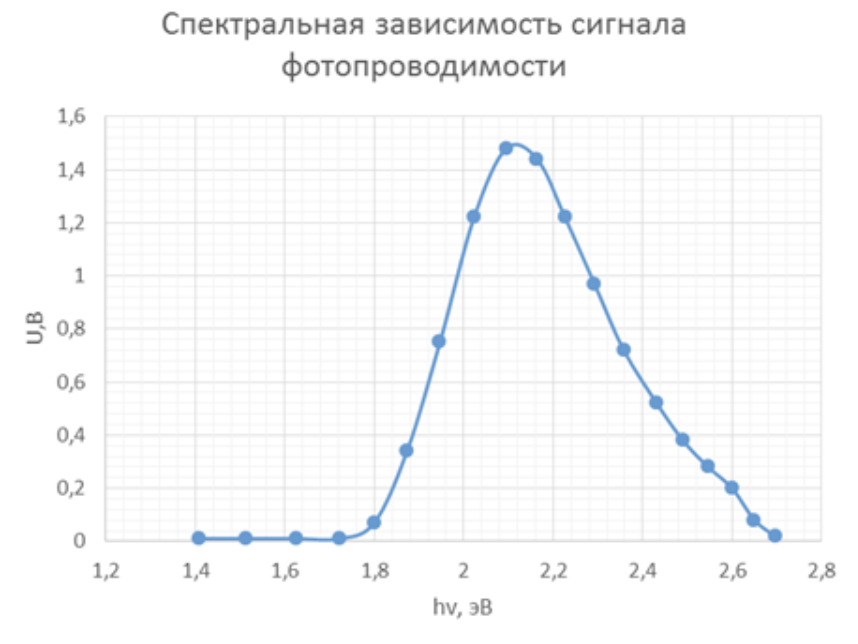
\includegraphics[scale = 0.6]{12.png}
        \caption{}
        \label{12}
    \end{figure} 
    Из графика зависимости коэффициента полгощения от энергии фотонов для кремния $K(h \nu)$ видно изменение оптических свойств, соответсвующее переходу из оптически тонкого состояни я в оптически толстое ($kd \sim 1$). При $K \approxeq 110\; cm^{-1}$, те $d \approx 91$ мкм.

    

\end{enumerate}



\end{document}